\documentclass[a0paper, portrait]{baposter}
\usepackage{graphicx}
\usepackage[english]{babel}
\usepackage{calligra}
%\usepackage[usenames,dvipsnames]{xcolor}


\begin{document}
\begin{poster}{
    % Poster Environment Options
    grid=false,
    columns=3,
    colspacing=1.0cm, % subject to change
    headerheight=0.1\textheight,
    background=plain,
    bgColorOne=white,
    eyecatcher=true,
    %Postbox environment options
    borderColor=black,
    headerColorOne=green,
    headerColorTwo=green,
    textborder = roundedsmall,
    headerborder=closed,
    headershape=rounded,
    headershade=plain,
    boxshade=none,
    linewidth=0.15cm
}
  % Eye Catch
  { 
\includegraphics[height=0.1\textheight]{ciidit.png} }
  % Title
  {\bf\textsc{Generation of Interactive Tag Clouds on Scientific Articles}} 
  % Author
  {
    Jes\'us Antonio Soto Vel\'azquez 
  }
  % Logo
  {
    
\includegraphics[height=8.0em]{uanl.png}
  }

  %%
  %% Poster Content
  %%

  % BOX1
  \headerbox{Intro}{name=intro, column=0, row=0} {
    Having a large collection of scientific articles grouped by topic, it was thought that the best way to visualize the main topics of these groups was through the use of tag clouds. At first glance, one is able to recognize what the articles in a certain group are about.
    \newline
   % \begin{center} 
      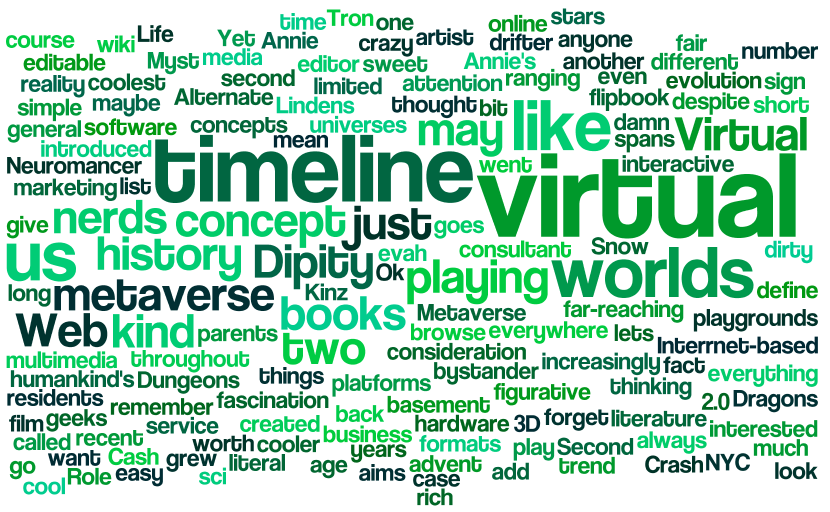
\includegraphics[height=0.1\textheight]{tagcloudsample.png}
    %\end{center}
    \newline
    A system that enables users to search through topics to find the corresponding group of articles and the involved artists is the {\bf objective}.The {\em key} is the interaction between the user and the tag cloud.
  }

  %BOX2
  \headerbox{Tackling the problem}{name=tech, column=0, below=intro} {
    Several aspects were taken into account when choosing the right information to put in the tag cloud, such as: \newline
    \begin{description}
    \item[Stopword filtering] Unimportant words in the given context were discaraded. Resolved with {\em String matching algorithms}.
    \item[Word stemming] Words with the same root were grouped together. Resolved with the {\em Snowball library}.
    \item[Language detection] Articles in other languages were to be excluded from the tag clouds. Resolved with the {\em language-detection library}.
    \item[The tag cloud] Manage structure and appearance of a tag cloud. Resolved with the {\em OpenCloud java library}.
    \item[Portability] As the intention was to reach as many users as possible, a web environment was chosen. Technologies used:{\em HTML5, CSS, Javascript, Servlets}
    \end{description}
  }
  %BOX3
  \headerbox{Initial solution}{name=initial, column=0, below=tech} {
    The initial solution made use of OpenCloud, a library in Java that facilitates the creation of tag clouds for the web. Using HTML and CSS, the tag cloud was given the desired styling and presentation.
    \newline
    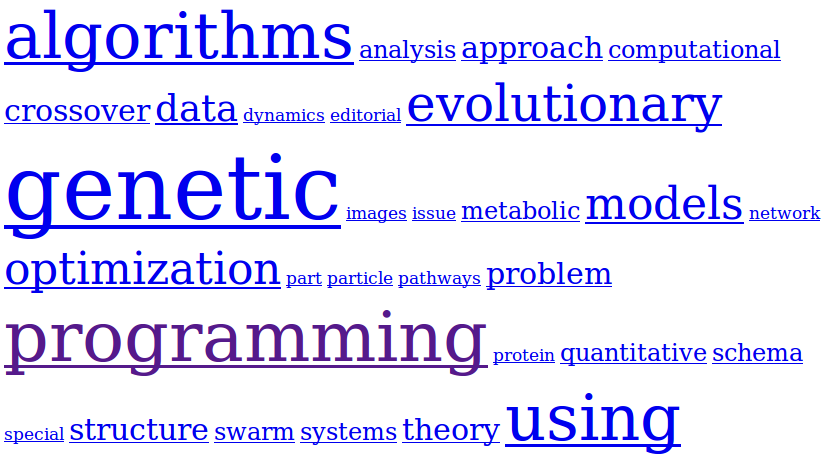
\includegraphics[height=0.1\textheight]{initial.png}
  }

  %BOX4
  \headerbox{Evolving approach}{name=evolve, column=1} {
    Having in mind the objective of the project, it was thought of a better way to position the items in the tag cloud to illustrate the relationship between similar and important topics in the group of articles. 
    \newline
    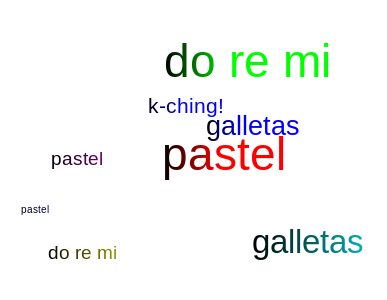
\includegraphics[height=0.1\textheight]{newcloud.png}
  }

  %BOX5
  \headerbox{Interacting with users}{name=interact, below=evolve, column=1} {
    The key to get more insight on the groups of articles was to allow the interaction with the tag cloud. An user can click an item in the tag cloud to find out who are the active researchers in that area, as well as discovering other topics they are involved in. HTML5 and its canvas was used to retrieve information on the clicked item.    
  }

  %BOX6
  \headerbox{Indexing articles}{name=index, column=2} {
To successfully deploy a system where topics inside the groups of articles were to be quickly searched, a structure known as an index was chosen. Each document is indexed so that the topics of the articles can be queried. 
The tool used to index the groups of articles, Solr, provides a simple interface between the data stored and the means of returning the desired information in a web environment.
  }
  
  %BOX7
  \headerbox{Future Work}{name=future, below=index, column=2} {
    Although the project focused on the many components involved, there is much work to be done to integrate these parts into a system for use in the web. Future work will focus mostly on deploying an architecture where the user inputs topics as queries, and the server processes these queries to return the tag clouds where such topics have been seen in certain groups of articles.
  }
  
  %BOX8
  \headerbox{References}{name=ref, below=future, column=2} {
    {\fontfamily{Calligra}\selectfont Charlie the unicorn for being the source of my inspiration.}
  }

\end{poster}
\end{document}
